%%%%%%%%%%%%%%%%%%%%%%%%%% lecture-7
\begin{frame}[shrink]
  \frametitle{lecture-7 主要内容}
  \framesubtitle{循环结构程序设计}
  \tableofcontents[hideallsubsections]
\end{frame}

\begin{frame}[shrink,fragile]{为什么需要循环控制}
\begin{itemize}
	\item 要向计算机输入全班50个学生的成绩;(重复50次相同的输入操作)
	\item 分别统计全班50个学生的平均成绩;	(重复50次相同的计算操作)
\end{itemize}
\begin{lstlisting}
float score1,score2,score3,score4,score5,aver; // 5门课成绩及平均成绩
// 输入第1个学生5门课的成绩
scanf(″%f%f%f%f%f″,&score1,&score2,&score3,&score4,&score5);
// 求第1个学生平均成绩
aver=(score1+score2+score3+score4+score5)/5;
printf(″aver=%7.2f″,aver); // 输出第1个学生平均成绩
// 输入第2个学生5门课的成绩
scanf(″%f%f%f%f%f″,&score1,&score2,&score3,&score4,&score5);
// 求第2个学生平均成绩
aver=(score1+score2+score3+score4+score5)/5;
printf(″aver=%7.2f″,aver);// 输出第2个学生平均成绩
...
\end{lstlisting}
\end{frame}

\begin{frame}[shrink,fragile]{用循环控制处理重复操作}
\begin{itemize}
	\item 要向计算机输入全班50个学生的成绩;(重复50次相同的输入操作)
	\item 分别统计全班50个学生的平均成绩;	(重复50次相同的计算操作)
\end{itemize}
\begin{lstlisting}
float score1,score2,score3,score4,score5,aver; // 5门课成绩及平均成绩
int i=1;         // 设整型变量i初值为1   
while( i<=50 )   // 当i的值小于或等于50时执行花括号内的语句
{
   scanf("%f%f%f%f%f",&score1,&score2,&score3,&score4,&score5);
   aver=(score1+score2+score3+score4+score5)/5; 
   printf("aver=%7.2f",aver);
   i++;  // 每执行完一次循环使i的值加1 
}   
\end{lstlisting}
\end{frame}

\section{$while(\text{表达式})\{ \cdots\}$}

\begin{frame}[shrink,fragile]{$while(\text{表达式})\{ \cdots\}$}
\begin{columns}
	\column{0.25\textwidth}
	\begin{lstlisting} 
    while( 表达式 )   
    {
       // 循环体
       执行多条语句;  
    }   
    \end{lstlisting}
	\column{0.3\textwidth}
	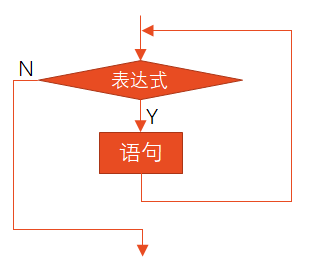
\includegraphics[scale=0.35]{while}
	\column{0.4\textwidth}
	\small
	\begin{block}{while循环特点}
		\small
		每轮循环: 首先判断表达式的值, 若``真" (以非0值表示)时,就执行循环体语句;为``假" (以0表示)时,就不执行循环体语句。
	\end{block}
\end{columns}
\begin{columns}
\column{0.45\textwidth}
\begin{block}{易犯错误}
\begin{lstlisting} 
while(表达式); 
{
   // 循环体
   执行多条语句;    
}
\end{lstlisting}
\end{block}
\column{0.45\textwidth}
\begin{block}{变体}
\begin{lstlisting} 
while(1)  
{
  if(表达式) break; // 退出循环
  执行多条语句;    
}
\end{lstlisting}
\end{block}
\end{columns}
\end{frame}

\begin{frame}[shrink,fragile]
$[$例5.1$]$ 求$1+2+3+\cdots+100$, 即$\sum\limits_{i=1}^{100}i$。
\begin{lstlisting}
   int i=1,sum=0;      //定义变量i的初值为1,sum的初值为0  
   while(i <= 100)     //当i>100,条件表达式i<=100的值为假,不执行循环体
   {                   //循环体开始
      sum=sum+i;          //第1次累加后,sum的值为1
      i++;                //加完后,i的值加1,为下次累加做准备
   }                   //循环体结束
   printf("sum=%d\n",sum); //输出1+2+3…+100的累加和                
\end{lstlisting}
\begin{enumerate}
	\setlength{\itemsep}{.2cm}
	\item 循环体如果包含一个以上的语句,应该用花括号括起来,作为复合语句出现。
	\item 不要忽略给$i$和$sum$赋初值,否则它们的值是不可预测的,结果显然不正确。
	\item 在循环体中应有使循环趋向于结束的语句。如本例中的$i++;$语句。如果无此语句,则i的值始终不改变,循环永远不结束。
\end{enumerate}
\end{frame}

\section{$do \{\cdots\} while(\text{表达式});$}

\begin{frame}[shrink,fragile]{$do \{\cdots\} while(\text{表达式});$}
\begin{columns}
	\column{0.25\textwidth}
	\begin{lstlisting} 
    do  
    {
      // 循环体
      执行多条语句;  
    } while( 表达式 );  
    \end{lstlisting}
	\column{0.35\textwidth}
	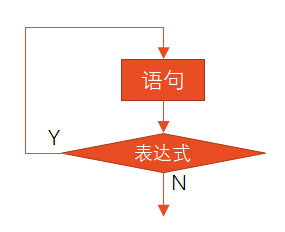
\includegraphics[scale=0.4]{dowhile}
	\column{0.4\textwidth}
	\begin{block}{循环特点}
		先无条件地执行循环体,然后判断循环条件是否成立。。
	\end{block}
\end{columns}
\begin{columns}
\column{0.45\textwidth}
\begin{block}{易犯错误}
\begin{lstlisting} 
do  
{
   // 循环体
   执行多条语句;  
} while( 表达式 )
\end{lstlisting}
\end{block}
\column{0.45\textwidth}
\begin{block}{变体}
\begin{lstlisting} 
do  
{
  执行多条语句;  
  if(表达式) break; // 退出循环  
} while(1);
\end{lstlisting}
\end{block}
\end{columns}
\end{frame}

\begin{frame}[shrink,fragile]
$[$例5.2$]$ 求$1+2+3+\cdots+100$, 即$\sum\limits_{i=1}^{100}i$。
\begin{lstlisting}
int i=1,sum=0;      //定义变量i的初值为1,sum的初值为0  
do     
{                   //循环体开始
   sum=sum+i;          //第1次累加后,sum的值为1
   i++;                //加完后,i的值加1,为下次累加做准备
}while(i <= 100);   //当i>100,条件表达式i<=100的值为假,不执行循环体
printf("sum=%d\n",sum); //输出1+2+3…+100的累加和                
\end{lstlisting}
\begin{enumerate}
	\setlength{\itemsep}{.2cm}
	\item 在一般情况下,用while()\{$\cdots$\}语句和用do\{$\cdots$\}while();语句处理同一问题时,若二者的循环体部分是一样的,那么结果也一样。
	\item 但是如果while后面的表达式一开始就为假(0值)时,两种循环的结果是不同的。
\end{enumerate}
\end{frame}

\begin{frame}[shrink,fragile]{$while(\text{表达式})\{ \cdots\}$与$do \{\cdots\} while(\text{表达式});$}
$[$例5.3$]$ 求$\sum\limits_{i=n}^{100}i$。考虑输入$n>100$时的情况,以下程序的不同。
\begin{columns}
\column{0.5\textwidth}
\begin{lstlisting}
int i,sum=0;
scanf("%d",&i);      
while(i <= 100)     
{                   
  sum=sum+i;          
  i++;               
}                  
printf("sum=%d\n",sum);               
\end{lstlisting}
\column{0.5\textwidth}
\begin{lstlisting}
int i,sum=0;
scanf("%d",&i); 
do     
{                   
  sum=sum+i;          
  i++;                
}while(i <= 100);   
printf("sum=%d\n",sum);                
\end{lstlisting}
\end{columns}
\end{frame}

\section{$for(\text{表达式1;表达式2;表达式3}) \{\cdots\}$}

\begin{frame}[shrink,fragile]{$for(\text{表达式1;表达式2;表达式3}) \{\cdots\}$}
\begin{columns}
\column{0.4\textwidth}
\begin{lstlisting} 
for(表达式1;表达式2;表达式3)
{
   // 循环体
   执行多条语句;  
}
\end{lstlisting}
$\equiv$
\begin{lstlisting} 
表达式1;
while(表达式2)
{
   // 循环体
   执行多条语句;
   表达式3;  
}
\end{lstlisting}
\column{0.4\textwidth}
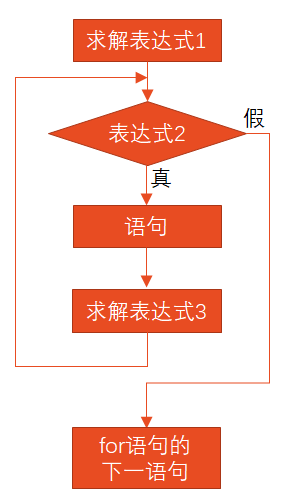
\includegraphics[scale=0.35]{for}
\end{columns}
\end{frame}

\begin{frame}[shrink,fragile]{$for(\text{表达式1;表达式2;表达式3}) \{\cdots\}$}
\begin{columns}
\column{0.25\textwidth}
\begin{lstlisting} 
for(表达式1;表达式2;表达式3)
{
   // 循环体
   执行多条语句;  
}
\end{lstlisting}
\column{0.3\textwidth}
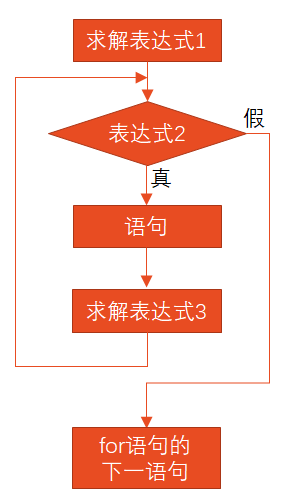
\includegraphics[scale=0.35]{for}
\column{0.45\textwidth}
\begin{itemize}
\item 表达式1: 设置初始条件,只执行一次。可以为零个、一个或多个变量(逗号隔开)设置初值。
\item 表达式2: 是循环条件表达式,用来判定是否继续循环。在每次执行循环体前先执行此表达式(包括第1次循环),决定是否继续执行循环。
\item 表达式3: 作为循环的调整,例如使循环变量增值,它是在执行完循环体后才进行的。	
\end{itemize}
\end{columns}
\end{frame}

\begin{frame}[shrink,fragile]{$for(\text{表达式1;表达式2;表达式3}) \{\cdots\}$, 省略表达式}
\begin{columns}%[T]
\column{0.3\textwidth}
\begin{lstlisting} 
int i;
for(i=0;i<=100;i++)
{
  printf("%d\n",i);
}
\end{lstlisting}
\column{0.3\textwidth}
\begin{lstlisting} 
int i=0;
for(;i<=100;i++)
{
  printf("%d\n",i);
}
\end{lstlisting}
\column{0.4\textwidth}
\begin{lstlisting} 
int i=0;
for(i=0;;i++)
{
  if(i>100) break;//退出循环
  printf("%d\n",i);
}
\end{lstlisting}
\end{columns}
\rule{\textwidth}{1pt} % 水平线
\begin{columns}%[T]
\column{0.3\textwidth}
\begin{lstlisting} 
int i;
for(i=0;i<=100;)
{
  printf("%d\n",i);
  i++;
}
\end{lstlisting}
\column{0.3\textwidth}
\begin{lstlisting} 
int i=0;
for(;i<=100;)
{
  printf("%d\n",i);
  i++;
}
\end{lstlisting}
\column{0.4\textwidth}
\begin{lstlisting} 
int i=0;
for(;;)
{
  if(i>100) break;//退出循环  
  printf("%d\n",i);
  i++
}
\end{lstlisting}
\end{columns}
\end{frame}

\section{循环的嵌套}

\begin{frame}{循环的嵌套}
\centering
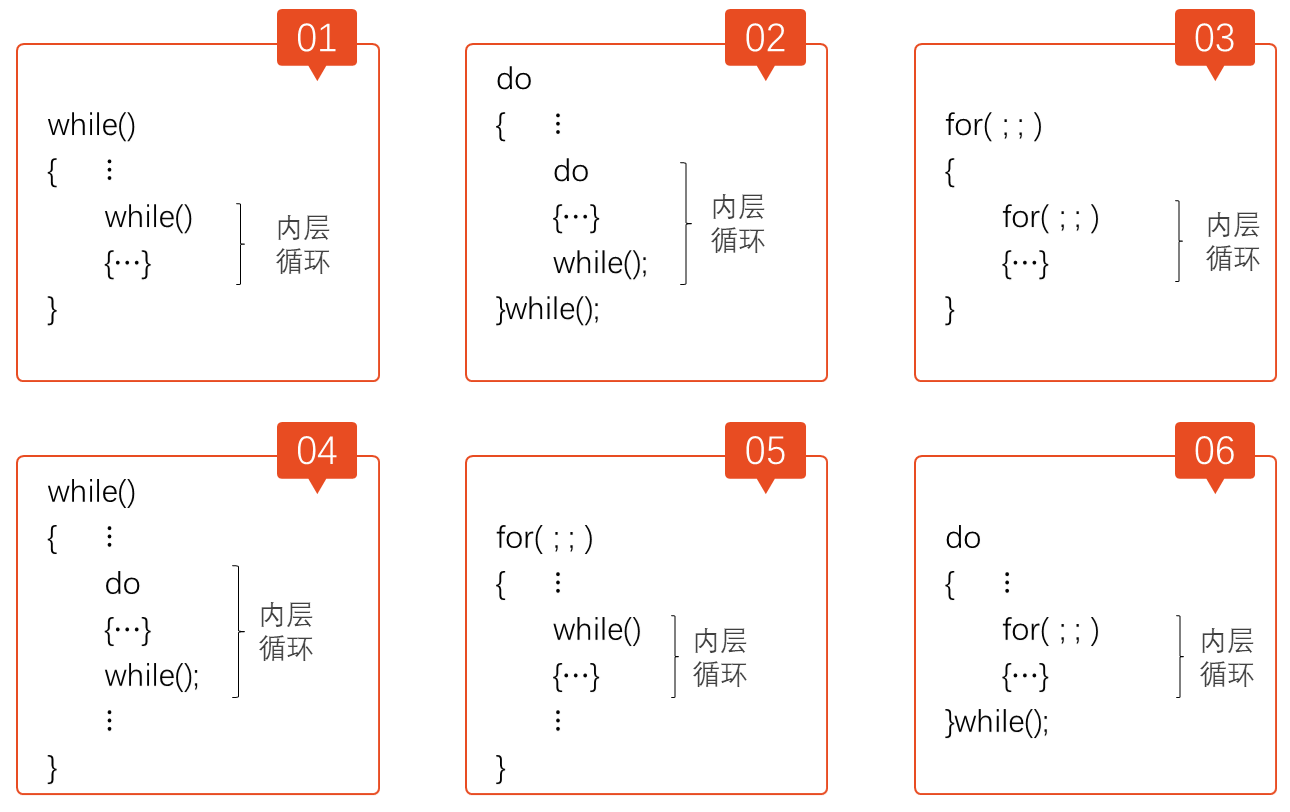
\includegraphics[scale=0.24]{whileWhile}
\end{frame}

\begin{frame}{几种循环的比较}
\begin{enumerate}
	\item 3种循环都可以用来处理同一问题,一般情况下它们可以互相代替。
	\item 在while循环和do…while循环中,只在while后面的括号内指定循环条件,因此为了使循环能正常结束,应在循环体中包含\textbf{使循环趋于结束的语句}(如i++等)。
	\item for循环可以在表达式3中包含使循环趋于结束的操作,甚至可以将循环体中的操作全部放到表达式3中(逗号隔开)。因此for语句的功能更强,凡用while循环能完成的,用for循环都能实现。
	\item 用while和do…while循环时,循环变量初始化的操作应在while和do…while语句之前完成。而for语句可以在表达式1中实现循环变量的初始化。
	\item while循环、do…while循环和for循环都可以用break语句跳出循环,用continue语句结束本次循环。	
\end{enumerate}
\end{frame}

\section{break,continue改变循环执行的状态}

\begin{frame}[shrink,fragile]{break,continue改变循环执行的状态}
\centering
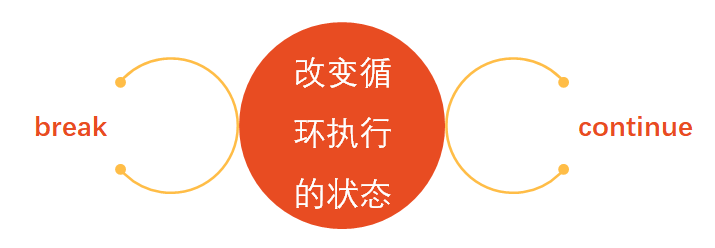
\includegraphics[scale=0.3]{breakContinue}
\begin{columns}[T]
\column{0.5\textwidth}
\begin{lstlisting}
while(表达式)
{
  printf("语句1");
  if(条件表达式) break; //提前终止循环
  printf("语句1");
}
\end{lstlisting}
\column{0.5\textwidth}
\begin{lstlisting}
while(表达式)
{
   printf("语句1");
   if(条件表达式) continue; //结束本次循环, 进入下轮循环
   printf("语句1");
}
\end{lstlisting}
\end{columns}
\end{frame}

\begin{frame}[shrink,fragile]{用break语句提前终止循环}
$[$例5.4$]$在全系1000名学生中举行慈善募捐,当总数达到10万元时就结束,统计此时捐款的人数以及平均每人捐款的数目。
\begin{lstlisting}
#define SUM 100000  //指定符号常量SUM代表10万
float amount,aver,total; 
int i;
for (i=1,total=0; i<=1000; i++)// 表达式1给多个变量赋初值,用逗号隔开。
{
  printf("please enter amount:");
  scanf("%f",&amount);
  total = total + amount; 
  if(total >= SUM) break; 
}
aver=total/i;
printf("num=%d\naver=%10.2f\n",i,aver); 
\end{lstlisting}
\textbf{\textcolor{blue}{注意: break语句只能用于循环语句和switch语句之中,而不能单独使用。}}
\end{frame}

\begin{frame}[shrink,fragile]{用continue语句提前结束本次循环}
$[$例5.4$]$要求输出100$\sim$200之间的不能被3整除的数。
\begin{columns}
\column{0.5\textwidth}
\begin{lstlisting}
#include <stdio.h>
int main()
{
  int n;
  for (n = 100;n <= 200;n++)
  {
    if (n%3==0) continue;
    printf("%d ",n);
  }
  printf("\n");
  return 0;
} 
\end{lstlisting}
\column{0.5\textwidth}
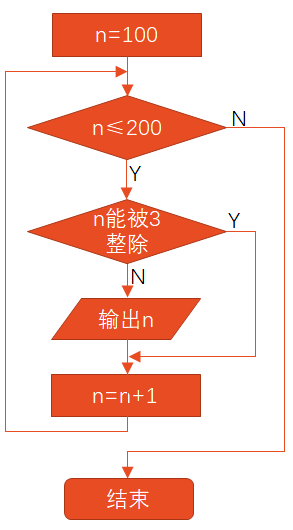
\includegraphics[scale=0.3]{for3}
\end{columns}
\end{frame}

\begin{frame}{break语句和continue语句的区别}
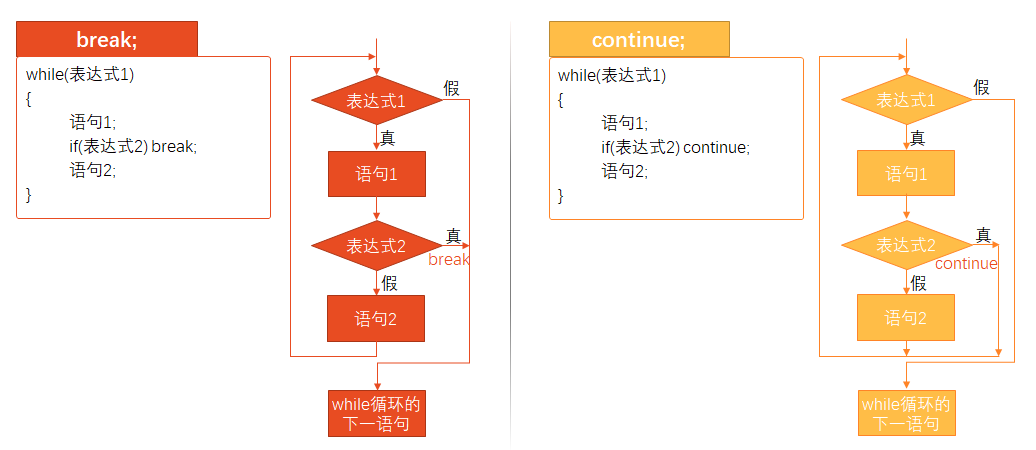
\includegraphics[scale=0.34]{forContinue}\\
\textbf{\textcolor{blue}{注意: continue语句只结束本次循环,而非终止整个循环。break语句结束整个循环,不再判断执行循环的条件是否成立。}}
\end{frame}

\begin{frame}[shrink,fragile]{break语句和continue语句的区别}
\small $[$例5.5$]$ 输出以下$4\times 5$的矩阵。
\begin{columns}
\column{0.5\textwidth}
\begin{lstlisting}
int i,j,n=0;
for(i=1;i<=4;i++)
{
  for(j=1;j<=5;j++,n++) //n用来累计输出数据的个数
  {
    if(n%5==0) printf("\n"); //控制在输出5个数据后换行
    if (i==3 && j==1) break;
    printf("%d\t",i*j);
  } 
} 
printf("\n");  
\end{lstlisting}
\column{0.5\textwidth}
\begin{lstlisting}
int i,j,n=0;
for(i=1;i<=4;i++)
{
   for(j=1;j<=5;j++,n++) //n用来累计输出数据的个数
   {
     if(n%5==0) printf("\n"); //控制在输出5个数据后换行
     if (i==3 && j==1) continue;
     printf("%d\t",i*j); // \t就是Tab键,是特殊字符,表示多个空格
   } 
} 
printf("\n");    
\end{lstlisting}
\end{columns}
\end{frame}

\begin{frame}{注意事项小结}
\begin{enumerate}
	\setlength{\itemsep}{.5cm}
	\item while( )\{ \}; do \{ \} while( ); for(;;)\{ \}执行顺序;
	\item 循环变量的开始和结束条件;
	\item 循环体是复合语句时,必须用\{ \}扩起来;
	\item 必要时,用break结束整个循环,用continue结束本次循环;
	\item 关键是找出循环规律,必要时设计流程图,指导代码实现。	
\end{enumerate}
\end{frame}